\section{Implementation} % (fold)
\label{sec:implementation}

Using the requirements set forth in Section~\ref{sec:dvpns} we can compile a list of contemporary technologies that can meet them and provide \acp{dvpn}. The protocols considered had to meet \ref{lst:num} criteria:
\begin{inparaenum}[\itshape 1\upshape)]
	\item can provide Ethernet \acp{ppvpn} between multiple sites, and
	\item protocol stack must be supported in hardware at time of writing.
	\label{lst:num}
\end{inparaenum}

MPLS - tag of traffic
VPLS - encapsulates Ethernet frames
RSVP - distributes labels downstream / ecmp / te
LDP - distributes labels upstream / ecmp
OSPF - learns topology of network
BFD - provide connectivity checks


PBB - tag traffic
IS-IS - learns topology of network
SPB - ecmp / te


what can provide what function for DVPNs?

\subsection{Contemporary Technologies} % (fold)
\label{sub:contemporary_technologies}

\subsubsection{\acs{spb}} % (fold)
\label{ssub:spb}

\ac{spb} is an evolution of the original \acs{ieee} 802.1Q \ac{vlan} standard. \ac{vlan} tags have been in use in the networking world for a long time and provide decent separation in campus networks. However, when \ac{vlan}-tagging was done at the customer network, the carrier couldn't separate the traffic from different customers anymore. This resulted in 802.1Qad or Q-in-Q which added an S-\ac{vlan} tag to separate the client \acp{vlan} from the \ac{sp} \acp{vlan} in the backbone. This was usable for the Metro Ethernet networks for awhile but when \acp{sp} started providing this services to more and more customers, their backbone switches could not keep up with the clients \ac{mac} addresses.

To provide the required \acs{mac} scalability problem \ac{pbb} (802.1Qay or \ac{mac}-in-\ac{mac}) was introduced. It encapsulates the whole Ethernet frame on the edge of the carrier network and forwards the frame based on the Backbone-\ac{mac}, Backbone-\ac{vlan} and the I-SID. The I-SID is a Service Instance Identifier, which with 24 bits is able to supply the carrier with 16 million separate networks. The downside of \ac{pbb} remained one that is common to all Layer 2 forwarding protocols: the possibility of loops. Preventing them requires \ac{stp} which will disable links to get a loop-free network. Disadvantages of \ac{stp} include the relatively long convergence time and inefficient use of resources due to the disabled links. This final problem was solved by using \acs{isis} as a routing protocol to distributed the topology and creating \acp{spt} originating from each edge device. This is called \ac{spb} or 802.1aq.

% EXPLAIN HOW IT CAN BE USED TO IMPLEMENT

% subsubsection spb (end)

\subsubsection{\acs{mpls}} % (fold)
\label{ssub:mpls}

\ac{mpls} is known for its scalability and extensibility. Over the past decade additions have been made to the original specification to overcome a plethora of issues within carrier networks. This initially started with trying to implement fast forwarding in legacy switches using labels (or tags) at the start of the frame \cite{tag-switching}. When this issue became surmountable using new hardware, \ac{mpls} had already proven to be capable of transporting a wide arrange of protocols on the carrier backbone network, all the while also providing scalability, \ac{te} and \ac{qos} features to the operators.

% EXPLAIN HOW IT CAN BE USED TO IMPLEMENT

\begin{figure}[!h]
	\centering
	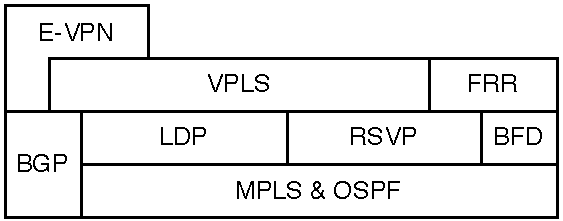
\includegraphics[width=7cm]{./includes/mpls-stack.pdf}
	\caption{Dependency stack of \ac{mpls}-related technologies.}
	\label{fig:mpls-stack}
\end{figure}

\begin{figure}[!h]
	\centering
	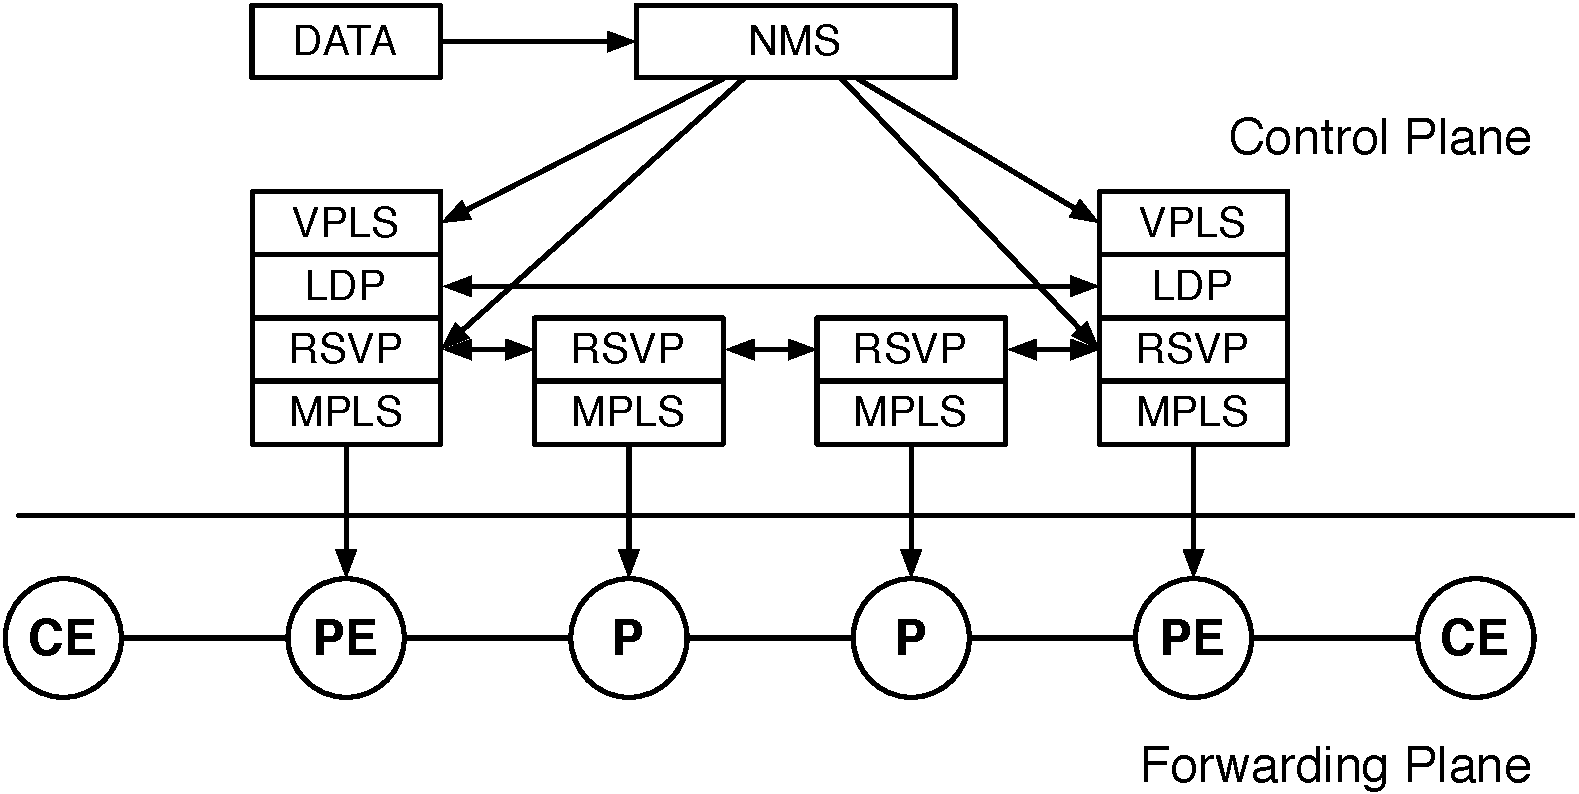
\includegraphics[width=9cm]{./includes/nms-stack.pdf}
	\caption{Provisioning a \ac{dvpn} using \ac{mpls}.}
	\label{fig:nms-stack}
\end{figure}

% subsubsection mpls (end)

% subsection contemporary_technologies (end)

\subsection{OpenFlow} % (fold)
\label{sub:openflow}

Section~\ref{sec:introduction} gave a short introduction into what \ac{sdn} and OpenFlow entail and what it promises in terms of cost savings and agility. \acl{sdn} is the general principle of designing flexible networks using open interfaces towards the hardware. The complete architecture is being standardized by the networking industry within the OpenDaylight project \cite{opendaylight}. Looking at OpenFlow itself from a more technical point of view, it boils down to a protocol used to program the forwarding plane in networking devices from a centralized server called the `controller'. 

The momentum that \ac{sdn} is getting might be explained by a general need for change in the networking industry. Operators primarily want to get more control over their networks, something which using the current stack of protocols is relatively complicated to get. The original \acs{osi} reference model \cite{zimmermann} touches on the ``Management Aspects'' of each layer in the model, a way for management entities in the highest layer to control the behavior of lower layers. Unfortunately in the swift evolution of \ac{tcp}/\ac{ip}, these management interfaces are often limited or absent all together. 

The OpenFlow controller provides operators with an alternative to these interfaces, namely a programmable forwarding plane. This gives them \ac{te} and \ac{qos} control by using custom applications to direct traffic through the network. 

The OpenFlow specification has been through a few revision since it was first proposed. In the first version tagging of traffic was only support using a single \acs{vlan} tag. Version 1.1 added matches for \ac{mpls} and Q-in-Q tags, and version 1.3 could also match \ac{pbb} tags. These features are essential for implementing \acp{vpn} because the traffic flows will need to be separated upon entering the carrier network. Also, with scalability in mind we do not want to learn the client \acsp{mac} in the core of the network.

Also not included in version 1.0 were mechanisms to allow for fast failover and \ac{ecmp}. These were added in version 1.1 by introducing logical groups of ports to which a flow entry can forward the frame. However, to support fast failover a \textsl{liveness monitoring} technique will need to be implemented supported by the switch. This could simply be the physical link state or more intricate tools, e.g.\ \ac{bfd}.

\begin{figure}[!h]
	\centering
	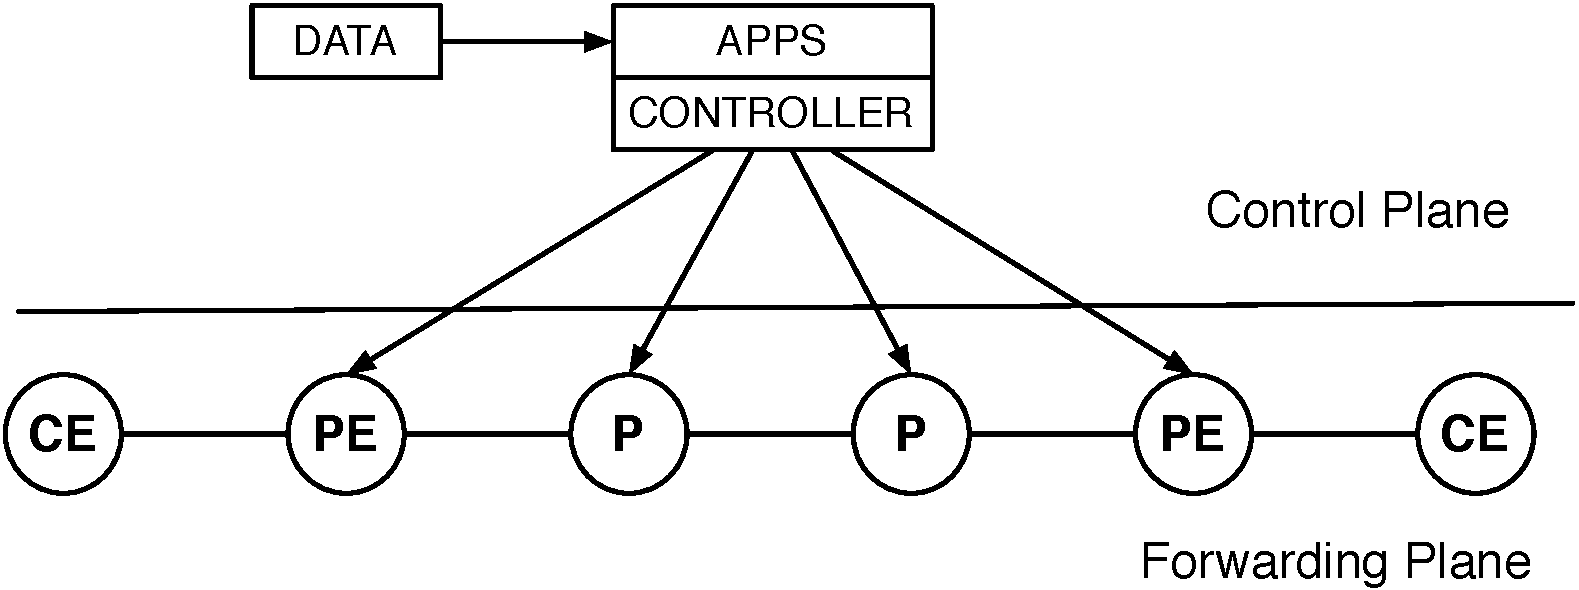
\includegraphics[width=9cm]{./includes/nms-stack-of.pdf}
	\caption{Provisioning a \ac{dvpn} using OpenFlow.}
	\label{fig:nms-stack-of}
\end{figure}

% subsection openflow (end)

The features and limitations of the three discussed technologies are given in Table~\ref{tb:reqs}. They are compared to the list of requirements as summarized in Section~\ref{sub:requirements}. Section~\ref{sec:results} will continue with an evaluation of the three architectures.

\begin{table}[h]
	\centering
	\begin{tabular}{r|lll}
	 & \acs{spb} & \acs{mpls} & OpenFlow / \acs{sdn}\\
	\hline
	Tagging of VPN Traffic & \acs{pbb} & \acs{vpls} & \acs{pbb} / \acs{mpls}\\
	MAC Scalability & yes & yes & yes\\
	Topology Discovery & \acs{isis} & \acs{ospf} & application\\
	Path Provisioning & \acs{spt} & \acs{rsvp} / \acs{ldp} & application\\
	Traffic Engineering & limited & \acs{rsvp} & application\\
	\ac{ecmp} & limited & yes & yes, using Groups\\
	\ac{bum} limiting & dependent on \acs{hw} & dependent on \acs{hw} & yes, using Metering\\
	Exchange \acsp{cmac} & no & E-VPN (draft) & application\\
	Traffic Rate Limiting & dependent on \acs{hw} & dependent on \acs{hw} & yes, using Metering\\
	Fast Failover & no & \acs{frr} & yes, using Groups\\
	\acs{oam} & 802.1ag & \acs{lsp} Ping / \acs{bfd} & application\\
	\hline
	Forwarding Decision & \acs{pbb} tags & \acs{mpls} labels & flow entry \\
	\ac{bum} traffic handling & flood & flood & sent to controller\\
	\end{tabular}
	\caption{Required features and corresponding available technologies.}
	\label{tb:reqs}
\end{table}

% section implementation (end)